%\documentclass[review]{elsarticle}
\documentclass[review]{elsarticle}
\usepackage{underscore}
\usepackage{tikz}
\usepackage{tikz-uml}
\usetikzlibrary{positioning}
\usetikzlibrary{calc}
\usetikzlibrary{shapes.misc}
\usetikzlibrary{through,arrows} % for circle of nodes ...
\usetikzlibrary{shapes.arrows, fadings}

\newif\ifsummary
\summarytrue % or \draftfalse
\summaryfalse % or \draftfalse

\usepackage{local-tikz-style}

\usepackage{lineno,hyperref}
\modulolinenumbers[5]

\newcommand{\cd}[1]{ {\it #1} }%

\journal{Journal of \LaTeX\ Templates}

%%%%%%%%%%%%%%%%%%%%%%%
%% Elsevier bibliography styles
%%%%%%%%%%%%%%%%%%%%%%%
%% To change the style, put a % in front of the second line of the current style and
%% remove the % from the second line of the style you would like to use.
%%%%%%%%%%%%%%%%%%%%%%%

%% Numbered
%\bibliographystyle{model1-num-names}

%% Numbered without titles
%\bibliographystyle{model1a-num-names}

%% Harvard
%\bibliographystyle{model2-names.bst}\biboptions{authoryear}

%% Vancouver numbered
%\usepackage{numcompress}\bibliographystyle{model3-num-names}

%% Vancouver name/year
%\usepackage{numcompress}\bibliographystyle{model4-names}\biboptions{authoryear}

%% APA style
%\bibliographystyle{model5-names}\biboptions{authoryear}

%% AMA style
%\usepackage{numcompress}\bibliographystyle{model6-num-names}

%% `Elsevier LaTeX' style
\bibliographystyle{elsarticle-num}
%%%%%%%%%%%%%%%%%%%%%%%

\begin{document}

\begin{frontmatter}

\title{Using ISO standards to design a metadata registry for climate data}
%%\title{Elsevier \LaTeX\ template\tnoteref{mytitlenote}}
%%\tnotetext[mytitlenote]{Fully documented templates are available in the elsarticle package on \href{http://www.ctan.org/tex-archive/macros/latex/contrib/elsarticle}{CTAN}.}

%% Group authors per affiliation:
\author{Martin Juckes}
%%\author{Elsevier\fnref{myfootnote}}
\address{Rutherford Appleton Laboratory, Didcot, UK}
%%\fntext[myfootnote]{Since 1880.}

%% or include affiliations in footnotes:
%%\author[mymainaddress,mysecondaryaddress]{Elsevier Inc}
%%\ead[url]{www.elsevier.com}

%%\author[mysecondaryaddress]{Global Customer Service\corref{mycorrespondingauthor}}
%%\cortext[mycorrespondingauthor]{Corresponding author}
%%\ead{support@elsevier.com}

%%\address[mymainaddress]{1600 John F Kennedy Boulevard, Philadelphia}
%%\address[mysecondaryaddress]{360 Park Avenue South, New York}

\begin{abstract}
The climate modelling community collaborate globally to generate a coordinated portfolio of climate simulations which serve to advance scientific understanding and to support the Assessment process of IPCC. 
The interoperability of data products among the participating institutions is guaranteed by a detailed specification of the parameters to be archived and the associated metadata requirements.
This paper looks at the potential for increasing interoperability towards users outside this core community by expressing metadata requirements through the language of ISO standards on metadata registries. 
\end{abstract}

\begin{keyword}
Data registry\sep
Climate data management
\end{keyword}

\end{frontmatter}

\linenumbers



%% standards references not set well as stands ... can modify the titles or look for other styles in article-header.

%% beging document is embedded in article-header
%%\begin{document}

\section{Introduction}\label{sec:intro}

The wide exchange of climate model output underpins a growing awareness of the severe challenges of accelerating climate change.
This paper considers one aspect of the standardisation work which is needed to ensure the timely distribution of
accessible data products: the specification of thousands of physical parameters calculated and shared from all participating
institutions. The specifications include definitions of parameters, technical metadata requirements and information on the intended use of 
the parameter.

The global policy framework for responding to the multiple threats and challenges of climate change
draws on regular assessments from the Intergovernmental Panel on Climate Change (IPCC) providing an overview of the state of knowledge
concerning the science of climate change. Projections of possible future outcomes from climate models based
on a range of different social and industrial actions provide the foundation for the assessment of the impact of future climate variability.
The climate projections come from multiple independent research institutions, in a global activity known as the
Coupled Model Intercomparison Project (CMIP).
This is an activity of World Climate Research Program (WCRP) which is overseen by the Working Group on Coupled Models (WGCM).
While the IPCC assessments are developed in a carefully designed framework agreed at an intergovernmental level, 
the climate projections being assessed are deliverd by the research community through a broad
range of independentally managed research programmes, projects and activities. Coordination is provided through two
expert panels set up by WGCM: the CMIP Panel and the WGCM Infrastructure Panel.

The public debates around climate variability focus on a handful of physical parameters, such as temperature, rainfall, and wind speeds.
The demand for thousands of physical parameters arises from the crucial need to understand the reliabilty of the climate model
output. The exchange of data serves not only to produce the headline graphs of rising temperatures, but also provides
the basis for a forensic examination of the processes represented by the models in order to assess their credibility
and guide future developments \citep[see][]{Eyring2016}. 

The scope of the physical processes covered by the climate models is rapidly expanding.
Setting the standards to encompass this scope in the context of an extensive community of independent research scientists
brings many organisational and technical challenges [[specify]].

This paper is not a formal plan for delivering services with agreement among the parties concerned: it is a provider perspective
on options for improving the accuracy and efficiency of the processes around the 

The CMIP6 Data Request \citep[DREQ][]{juckes2019disc} provides detailed technical specifications of thousands of
climate parameters which are being
archived by climate modelling centres around the world as part of a global effort to update the set of reference
climate simulations which guide global policy on climate change mitigation and adaptation. 

The DREQ is part of a range of infrastructure projects \citep{Balaji2018}. See also ES-DOC \citep{pascoe2019disc}.

The DREQ is built on domain standards which have evolved with the CMIP project. In this paper we explore the
feasibility and potential benefits associated with expressing these specifications through ISO standards. 

The work cuts across a range of standards which are introduced in Section \ref{sec:iso} below, covering aspects of geospatial referencing, physical quantities, and the organisation and processes inherent in running a registry of metadata specifications. 

The expected benefits will be both in terms of inter-operability with other standards which deal with environmental information and also in terms of learning from and exploiting practises which are embedded in the ISO standards. 

We look at three principle areas of the activity.

Firstly, the description the overall orangisational structure. 

Secondly, community interaction which involves a broad and rapidly growing network,
with participants from hundreds of institutions and dozens of countries. The structure has evolved organically, always pressured by the rapid 
expansion of the global climate modelling activity and the societal pressures associated with growing awareness of the
risks posed by anthropogenic climate change. One of the consequences of the broad and loosely
coordinated collaboration is that names of some contributors are only recorded in email chains or online discussion.

Finally, the Information Technology.
The DREQ includes thousands of different quantities, 
all of which are defined in and registered in the CF Convention. In order to increase interoperability with
other communities this paper develops a mapping from the terms in the data request to ISO standard quantities.
We we also consider the definition of data types, including specification
of multi-dimensional arrays which combine geospatial coordinates with additional domain specific dimensions.

\begin{figure}[h]
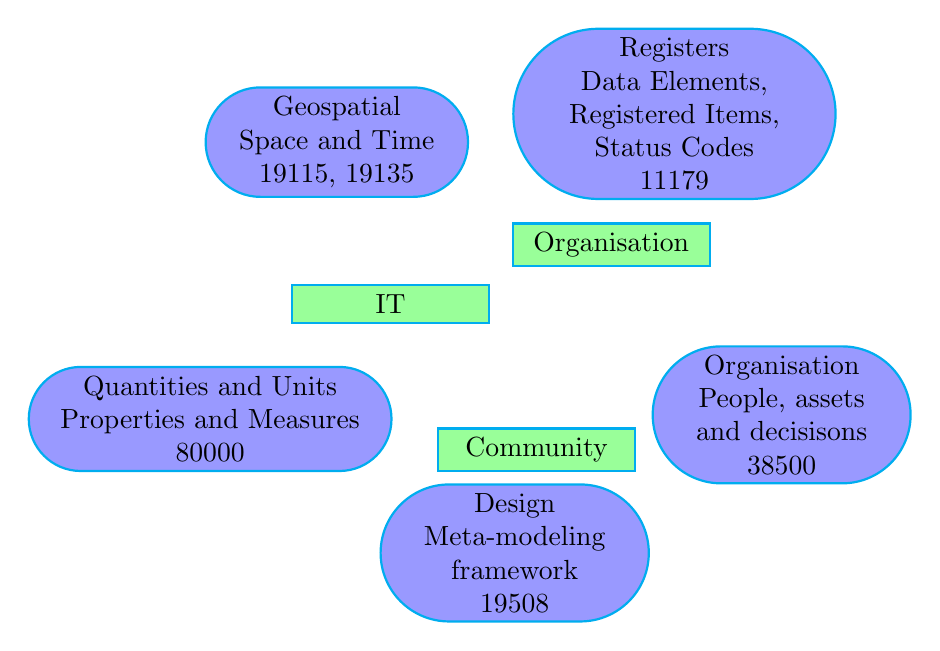
\begin{tikzpicture}[
  thick,
  every pin edge/.style={<-},
  >=latex,
  declare function/.list={
    outerR=2.0;,
    innerR=1.6;,
    angleofNode(\a)=\a/5*360-90;},
  std/.style={rounded rectangle, align=center, fill=blue!40, draw=cyan},
  chpt/.style={rectangle, minimum width=2.5cm, align=center, fill=green!40, draw=cyan}
  ]

\node [circle through=(0:outerR)] (c) {};
\node [circle through=(0:innerR)] (d) {};

%%\node[draw,chpt,anchor=90] at (d.40) {Organisation};
%%\node[draw,chpt,anchor=210] at (d.160) {IT};
%%\node[draw,chpt,anchor=330] at (d.270) {Community};
\node[draw,chpt] at (d.40) {Organisation};
\node[draw,chpt] at (d.170) {IT};
\node[draw,chpt] at (d.280) {Community};

\node[draw,std,anchor=angleofNode(2.5)] at (c.{angleofNode(0)}) {Design\\Meta-modeling\\framework\\19508};
\node[draw,std,anchor=angleofNode(3.5)] at (c.{angleofNode(1)}) {Organisation\\People, assets\\and decisisons\\38500};
\node[draw,std,anchor=angleofNode(4.5)] at (c.{angleofNode(2)}) {Registers\\Data Elements,\\Registered Items,\\Status Codes\\11179};
\node[draw,std,anchor=angleofNode(0.8)] at (c.{angleofNode(3)}) {Geospatial\\Space and Time\\19115, 19135};
\node[draw,std,anchor=angleofNode(1.5)] at (c.{angleofNode(4)}) {Quantities and Units\\Properties and Measures\\80000};

\end{tikzpicture}
\caption{The five core standards explored in this paper. The scope of these five standards overlaps in many areas, but
there do not appear to be any inconsistencies in the application discussed here.}
\label{fig:pentad}
\end{figure}


\subsection{Exploiting the International Standards Organisation [ISO]}\label{sec:iso}

The ability to discuss the whole range of issues from governance to comprehensive technical details is a valuable 
strength of the ISO standards. This is of particular relevance in the context of a metadata registry which is
constructed through wide community engagement. Different categories of technical information require different
forms of approval and harmonisation. This paper aims to clarify the procedures, roles and responsibilities
through the ISO framework.



The main pillars of the work are the standards listed here: 

\begin{itemize}
\item QU Quantities and Units: Parts 1: General \cite{iso80000-1},
         3: Space and Time \cite{iso80000-3}, 4: Mechanics \cite{iso80000-4}, 5: Thermodynamics \cite{iso80000-5},
         7: Light and Radiation \cite{iso80000-7}, and  9: Physical Chemistry and Molecular Physics \cite{iso80000-9}.
%%\item QU-ST Quantities and Units (80000-3 {Space and Time})
%%\item QU-ME Quantities and Units (80000-4 {Mechanics})
%%\item QU-TH Quantities and Units (80000-5 {Thermodynamics})
%%\item QU-AC Quantities and Units (80000-7 {Light and Radiation})
%%\item QU-NP Quantities and Units (80000-9 {Physical Chemistry and Molecular Physics})
\item GIM Geographic Information --- Metadata (19115-1 \cite{iso19115-1})
\item GIP Geographic Information --- Procedures (19135-1 \cite{iso19135-1})
\item MDR Metadata Registries (11179)
\item ITG Governance of Information Technology \cite{iso38500}
\item EIF Enterprise integration — Framework for enterprise modelling, \cite{iso19439} 
\item EIC Enterprise integration — Constructs for enterprise modelling, \cite{iso19440}
\item MOF OMG Meta Object Facility \cite{iso19508}
\item GPD General Purpose Datatypes \cite{iso11404}
\end{itemize}

[[literature survey needed]]

\cite{sinaci2013} describes the ise of ISO 11179 to facilitate exchange across clinical work and care domains.
5 odp viewpoints

\cite{mcclatchkey2018} discusses the use of a MOF layered metamodel to design a systematic approach to collecting provenance information in a distributed software system. Here we are looking at a somewhat different problem of capturing provenance information arising from multiple interacting science teams and institutions. From a modeling perspective, there is some similarity. Setting out the requirements for provenance collection clearly in the upper layers of the m-cake provides a systematic framework for embedding the functionality consistently in a range of different artefacts at the workflow implementation layer. 


\section{Layering the Technical and Organisational Design}

\subsection{Modeling approach}

The Object Management Group (OMG) Meta Object Facility (MOF) \citep{iso19508} will be applied, so that the structure
can be specified in 4[[?]] layers. 

Firstly, the MOF layer (this section) defining the use of MOF, decsribing the objectives of the four layers used, and additional 
framing assumptions.

The second layer specifies the overall technical and organisational structures of the registry, exploiting the Metadata Registries
standard \citep{iso11179-1}.

The third layer specifies the structure of the registers within the registry, the organisational units associated with them, and
their requirements.

Finally, the fourth layer includes the contents of the registries.

\subsubsection{The apex concept}

In MOF, the properties of the apex concept are inheritted by all other classes in the system.

\subsubsection{The self-descriptive registry}

\paragraph{ISO 11179} \citep[Metadata Registry][]{Pon2009} provides a framework for the organisational
structure of a metadata registry and for the technical specifications of the registers within that registry.
Critically, this clarifies the decision processes and responsibilities surrounding the registration of new items. 

The ISO 11179 standard requires that all concepts used in the metadata registers should have their metadata declared
in a manner consistent with the standard. Hence, the registry can be used to maintain a record of the organistational
structure of the registry. The creation of a \cd{MDR_registeredItem} is defined by 11179 in terms of a set of sub-classing operations:
\begin{quote}
\cd{MDR_identifiedItem} $\to$ {MDR_registeredItem} $\to$ {MDR_AdministeredItem}.
\end{quote}

[see 13.1.8 of UML2 \citep{uml2}: "Stereotype is a kind of Class that extends Classes through Extensions".]
In order to build this structure into a model which combines features from other standards we will define procedural \cd{stereotypes} on
the inheritance/generalization relation:
\begin{itemize}
\item \cd{identify}: create a sub-class that conforms to \cd{MDR_identifiedItem};
\item \cd{register}: create a sub-class that conforms to \cd{MDR_registeredItem};
\item \cd{administer}: create a sub-class that conforms to \cd{MDR_administeredItem}.
\item \cd{attach}: create a sub-class that conforms to \cd{MDR_attachedItem}.
\item \cd{XXadopt}: create a sub-class that conforms to \cd{MDR_designatableItem}.
\item \cd{rdef}: create a sub-class that conforms to \cd{MDR_dataElement}.
\end{itemize}

The scope and intent of these stereotypes is defined here, the technical specifications will be in layer [[apex-1]].

[[not clear if "Extension" is an acceptable relationship across MOF layers ...]]

[[NB: \cd{UML::valueSpecification} "may reference an instance when evaluated"]]

%%\begin{figure}[h]
%%\begin{tikzpicture}
%%\umlsimpleclass[sc1,y=0]{Apex}
%%\umlsimpleclass[sc1,y=0,x=5,type={concept}]{}
%%\end{tikzpicture}
%%\end{figure}

Enumerations are used to classify data element concepts, such as the time interval between data fields in a dataset.
In DREQ many of the enumerations used in this way are themselves the product of a community registration process. 
In ISO 11179, however, the elements of an enumeration used to define \cd{MDR_Value_Meaning} must be designatable items
rather the registered items. The \cd{XXadopt} stereotype is introduced to deal with this. An instantiation with stereotype \cd{XXadopt}
may be used to create a \cd{MDR_designatableItem} from a \cd{MDR_registeredItem} or \cd{MDR_administeredItem}.
[[not clear that generalization is the best approach here ... may be better to associate with the registered item]]

This allows a separation of procedures and governance between the registration and administration process for such items and that of the
other items in the registry which depend on designatable items for their definitions. 

In practice, the procedures for \cd{XXadopt} are likely to run in parallel to \cd{register} and \cd{administer}. The split between these
two concepts in meta-model resolves a potentially confusing governance structure when item $X$ is defined in
terms of items $A$, $B$ and $C$ which all have distinctive governance and management workflows. 

The \cd{rdef} stereotype generates a data element class, which may be used to specify the syntax for representing, for instance,
\cd{ITG_decision_centres}.


\subsection{Technical and Organisational Structures}

The ISO 38500 standard on governance is designed to deal with corporate governance structures, but achieves its purpose through 
a high degree of flexibility. The ability to define cascading chains of responsibility, with the option, at each stage, for 
organisational units to define their own internal governance structures, makes it suitable for the highly non-corporate 
structure that assembles the CMIP Data Request.

What 38500 does specify is key concepts of an organisational system (decision centres, assets, competencies etc) and
a framework for describing them and their connections. In this implementation, these organisational classes will inherit
the basic aspects governing status etc from the 11179 apex concept.

In addition, the generalization with \cd{administer} stereotype
will be used to generate a suite of 

\subsubsection{stereotypes}

\cd{identify} adds attribute identifier referencing a \cd{MDR_Scoped_Identifier} [MDR, part 3, chapter 7, figure 5] instance.

Specialisations: require one \cd{MDR_Scoped_Identifier} in the registry namespace. 

\cd{register} adds \cd{MDR_submission_record}. A registered item may also be a designatable item.

\subsubsection{Principles of the technical schema}

Technical specifications are sometimes split between a "schema" and "vocabularies", with vocabularies containing extensible lists of
terms relevant to a specific domain or technical application. The vocabularies may be structured according to schema, and the "schema" may contain lists, so the distinction is somewhat arbitrary. 

%%Here, we draw the distinction between a aggregating schema, which is defined to include additional information
Here, the distinction will be betweem register with MDR designated items and one with MDR registered items.


\subsection{Actors and Registers}

\subsection{Decisions and Data Elements}


\ifsummary
 %% [additional content omitted]
\else
\section{Overview of the metadata structures}

\subsection{Activities and Roles}\label{sec:roles}

\documentclass[tikz,border=10pt]{standalone}
\usepackage{tikz-uml}
\usetikzlibrary{positioning}
\usetikzlibrary{calc}

\tikzset{
  pck/.style = {
    minimum width = 3cm,
    node distance=2in,
    },
  note/.style = {
    width = 6cm,
    }
  }

\begin{document}

\begin{tikzpicture}

\begin{umlsystem}[x=4, fill=red!10]{The data request registry}
\umlusecase [name=AA] {Registry}
\umlusecase [below = 1cm of AA, name=A] {Register Collection}
\umlusecase [below = 1cm of A, name=B] {Register}
\umlusecase [below right = 0.5cm and 1cm of B, name=dec] {Item Specs}
\umlusecase [below left = 0.5cm and 1cm of B, name=ri] {Registered Item}
\umlusecase [x=2cm,y=-3cm, name=mon] {Monitor}
\end{umlsystem}

\umlactor[x=-2cm,y=0.5cm]{registrar}
\umlactor[x=-2cm,y=-1.5cm]{programme}
\umlactor[x=-2cm,y=-3.5cm]{pi}
\umlactor[x=-2cm,y=-5.5cm]{experts}
\umlactor[x=8cm,y=-3cm]{oversight}

%% would be nice to place stereotype above line ... probably need to change anchor .... occurs dozens of times in style file
%% should be straight mapping of code used for "stereo pos"
%% can use arg1, arg2, mult1, mult2 for additional info, but quickly becomes crowded
%%
\umlassoc[draw=black!50, very thick, arg1=operate,stereo=own]{registrar}{AA}
\umlassoc[arg1=govern,stereo=coordinate]{programme}{A}
\umlassoc[arg1=define,stereo=ipr]{experts}{ri}
\umlassoc{pi}{B}


\end{tikzpicture}

\end{document}



\subsection{Metadata Packages}\label{sec:packages}

\begin{figure}[p]
\begin{tikzpicture}


\begin{umlpackage}[fill=green!20]{Metadata}
\begin{umlpackage}[]{Parameters}
\umlsimpleclass[sc1,y=0]{units}
\umlsimpleclass[sc1,y=-0.8cm]{quantities}
\umlsimpleclass[sc1,y=-1.6cm]{constraints}
\umlsimpleclass[sc1,y=-2.4cm]{variables}
\end{umlpackage}

\begin{umlpackage}[]{Data Axes}
\umlsimpleclass[sc1,x=5cm,y=0]{axes}
\umlsimpleclass[sc1,x=5cm,y=-1cm]{coordinates}
\umlsimpleclass[sc1,x=5cm,y=-2cm]{configurations}
\end{umlpackage}

\begin{umlpackage}[]{Data Types}
\umlsimpleclass[sc1,x=5cm,y=-4.6cm]{\detokenize{data-type}}
\umlsimpleclass[sc1,x=5cm,y=-5.4cm]{spatial-grid}
\umlsimpleclass[sc1,x=5cm,y=-6.2cm]{temporal-grid}
\umlsimpleclass[sc1,x=5cm,y=-7cm]{\detokenize{cell-methods}}
\end{umlpackage}

\begin{umlpackage}[]{Request}
\umlsimpleclass[sc1,x=0cm,y=-4.6cm]{variable-group}
\umlsimpleclass[sc1,x=0cm,y=-5.4cm]{experiment-group}
\umlsimpleclass[sc1,x=0cm,y=-6.2cm]{objective}
\begin{umlpackage}[fill=black!10]{Choices}
\umlsimpleclass[sc1,x=0.4cm,y=-8.0cm]{options}
\end{umlpackage}
\end{umlpackage}

\begin{umlpackage}[]{Imports}
\umlsimpleclass[sc1,x=0cm,y=-10.2cm]{MIP}
\umlsimpleclass[sc1,x=0cm,y=-11cm]{standard-name}
\umlsimpleclass[sc1,x=5cm,y=-10.2cm]{experiment}
\end{umlpackage}


\end{umlpackage}

%%% Request .. linking
%%% Experiment ... [obsolete ... only need a class with links to experiments]
%%% Data types (structure).
%%% Data axes (structure).
\end{tikzpicture}
\caption{The metadata package is split into 5 sub-packages characterised by different harmonization and conformance requirements and mechanisms.}
\label{fig:packages}
\end{figure}



\begin{tikzpicture}
%%\draw[cyan] (0,0) -- (12,0) -- (12,-5.5) -- (0,-5.5) -- cycle;

\node [text01,fill=cyan,text width=5.0cm,align=left,anchor=north west]  (text1) {
{\centering \bf Data Element\par} Configured Variable
};

\node at (text1.south) [
    right color=blue!50!cyan,
    single arrow,
    anchor=north,
    minimum height=1cm,
    inner sep=4pt,
    shading angle=90+60,
    rotate=90
] {};

\node [text01, text width=5cm,align=left, anchor=south west] (object) at ($(text1.north west) + (0.,1.)$) {
{\centering \bf Object\par} model component being described};

\node [text01, text width=5.5cm, align=left,anchor=south west] (par) at ($(text1.north east) + (0.,1.)$) {
{\centering \bf Property\par} the quantity being reported};

\node [text01, text width=5.5cm, align=left,anchor=west] (cd) at ($(text1.east)+(0.4,0.)$) {
{\centering \bf Generic processing\par} applied (spatial averaging, masking)};

\node [text01, text width=6.cm,align=left, anchor=north] (rqv) at ($(text1.south) + (0.,-.5)$) {
{\centering \bf Data Type\par} organisation of data values};

%%\draw[blue]
   %%($(sn.south)+(-1.,0)$) edge (text1.north)
   %%(var.west) edge ($(text1.east)+(0.,.2)$)
   %%(cmv.west) edge ($(text1.east)+(0.,-.2)$)
   %%($(rqv.north)+(-1.,0)$) edge (text1.south);
   
\end{tikzpicture}

\subsection{The Metadata Region of MDR}\label{sec:mdrmdr}

MDR-3 [How to refer?] provides the framework for specifying the metadata requirements for "registered items". In this case the objective is to specify the requirements for datasets which will be archived and distributed through the ESGF distributed archive. The \cd{MDR:Data Entitity} class which provides the registry component of the specifcations of these datasets corresponds to the \cd{DREQ:CMORvar}, a record defining a physical variable sepcified as a mutli-dimensional field spanning time, space and potentially, other dimensions
such as wavelength, land cover type, ...

The \cd{DREQ:CMORvar} defines a range of properties such as the temporal sampling frequency and spatial processing requirements (e.g. masking and averaging), in addition to the structure of the field and the specification of the physical property.

In the new framework, these metadata elements are distributed among \cd{datatypes}, \cd{classifications}, \cd{descriptions}, \cd{value domain subsets} [[not sure if the last is needed]]

The information relevant to the \cd{datatype} is specified in terms of concepts from the CF Conventions which build on the NetCDF data model of arrays, dimensions and attributes.


\section{Quantities and Units of Measure}

The concept of "quantity" is discussed in 19115, 11179 and 80000 (where it is the main focus of the standard). In all cases, a "quantity" is physical property which can be expressed via a measure.

The 19115 and 80000 define a range of specific quantities, and 11179 defines a framework for defining additional quantities. There is some
duplication between 19115 and 80000. Where possible we will use terms defined in 19115.

In both 19115 and 80000, the quantities defined generally have a broader scope that the variables defined in DREQ. For instance, the ISO 80000 quantity "Thermodynamic Temperature" corresponds to 33 different DREQ variables, such as "Near-Surface Air Temperature", "Temperature at Snow-Ice Interface".

There are 7 quantities from 19115 which are used (implicitly) in DREQ: angle, scale, distance, speed, area, volume, weight.

From 80000 the following: acceleration, time (duration), pressure, surface density, mass density, kinematic velocity, mass flow rate,
heat flow rate, density of heat flow rate, Celsius temperature(*), thermodynamic temperature, attenuation rate, mass fraction,
volume fraction, amount-of-mass fraction, amount-of-substance concentration.

These come from parts 3 (Space and Time), 4 (Mechanics), 5 (Thermodynamics), 7 (Light and Radiation) and
9 (Physical chemistry and molecular physics) of the standard.

(*) "Celsius temperature" could, according to the guidance given in ISO 80000, be considered as the same quantity as thermodynamic temperature. They only differ by a fixed offset.

The parameters in DREQ which do not appear to fit any of the specific quantities defined in ISO 11179 or ISO 80000 will be defined covered by defining new quantities as registered items in a consistent style and granularity. For instance, energy flow, temperature flux, stress, pressure tendency. 

In this way, it is possible to express the portfolio of parameters in around 100 quantities. Labelling the parameters with appropriate ISO quantities is likely to increase interoperability with other archives supporting fields, such as engineering or medicine, which may be involved in climate mitigation, adaptation or emergency response.

\section{Data Types}

The aim here is to establish a pathway to formal description. Implementation will continue to be via the CF and NetCDF structures.

It would be possible to develop a complex data type representing the full range of information required in a dataset. This consists of the required data array, the coordinates used to represent the data, and ancillary variables. 

An alternative approach is to represent the data requested as a MDR_data_entity with associated MDR_sub_data_entity concepts, such that each individual element corresponds to a single array of data.

This latter approach conforms to GI-MD. 

The top level data entity is a record specifying the dimensions of all the required arrays, some of which may be user specified.
e.g.
\begin{verbatim}
parametric data type: 
      type dimensions (lat: integer, lon: integer, time: integer ) = 
             record ( lat, lon, time, bnd=2);
\end{verbatim}
or perhaps, the data array ...
\begin{verbatim}
parametric data type:
      type data (lat: integer, lon: integer, time: integer ) =
             array ( 1..lat, 1..lon, 1..time) of real(8,64);
\end{verbatim}


The data field itself will then be held in a sub data entity,
\begin{verbatim}
parametric data type: type data = array (1...PA_time,1...PA_lon,1...PA_lat) of real(8,64);
\end{verbatim}

Additional sub-data entity elements will contain data for the dimensions and the ancillary variables.
This approach allows a fairly direct mapping of DREQ records into data entity concepts, but draws the \cd{dimensions}/\cd{data} data type into the 
top level data entity.

At this point the details of the mapping are not as important as the demonstration that the mapping is feasible. 


Base data types are perhaps more easily specified in CDL, but need to define a templating syntax. - use PEP 3101.
The values to be replaced are placed in braces, e.g. "{n:d}" should be replaced by the value of "n" using the formatting designated by "d" (a "decimal integer").



%% perhaps a table of class vs. attribute list {as itemize env}, showing data type and attributes. e.g. long_name : c"Near Surface Air-Temperature", where the 'C"..."' denotes a data entity with value given by the string

This extends \cd{MD_Dimension}

\begin{verbatim}
bounded latitude (n:integer,data:sequence) {
dimensions:
  integer lat = {n};
variables:
  double lat(lat);
     lat.standard name = "latitude";
     lat.units = "degree north";
     lat.long name = "latitude" ;
     lat.bounds = "lat bnds";
     lat.axes = "Y";
data:
  lat = {data};
}
\end{verbatim}
Note that in order to apply the PEP 3101 templating rules \verb+sequence+ would need to be expressed as a string.

The "data" needs to be expressed as a string .... not really what we want to say.

This can be expressed in the language of 11404:

\begin{verbatim}
parametric data type: type bounded latitude(values: sequence of (real(256,64) ) = \
      record (values,name: "lat", \
             long name: "latitude", \
             lat.bounds,..) ;
\end{verbatim}


The \cd{NetCDF:double} datatype corresponds to ISO 11404 \cd{real(2,64)}, i.e. 64-bit floating point. The remaining parameters are key-value pairs which define the physical
interpretation of the datatype through the CF Convention.

With this approach, however, the attributes \cd{lat.units} etc become external to the administrative structure of the registry, only the bundled entity 
is explicitly represented.

Express Datatype as a subclass of {\cd MDR:Concept} and define records to accomodate ....

The required data type elements will be (1) simple dimension, bounded dimension (inc. coordinate), fixed simple dimension, (4) fixed bounded dimension.

There are 35 land surface types used to express masking requirements of data. Desirable to move these to a \cd{mask} record, and express the CMOR grid table via a method of the registry. 

Similarly, there are a significant number of ancillary variables ("a", "b", etc) which should be expressed in the data type. Also "orog", which is a 2-d field.

.e.g \cd{hybrid height half} requires \cd{a, b, a bnds, b bnds, orog}.

The bounds variables have dimensions (n,2), and the orog variable is the shape of the spatial grid.

We can, however, express the fact that "level" must be one of "hybrid half height, alternate hybrid sigma, ...".


\begin{verbatim}
parametric data type: type values_type(n: integer) = array (1...n) of real(8,64);

parametric data type: type regular_longitude(m: integer) = record (values(n),name,long_name,bounds,..) ;
parametric data type: type regular_lat_lon(n: integer, m: integer) = record (values(n,m),name,dimensions(regular_latitude(n),regular_longitude(m));
type name = string-literal selecting ("latitude");
\end{verbatim}


11179 allows data types to be specified via a reference to a document.

Here, we use the notation of 11404 to specify the datatypes, since the underlying standards do not provide a formal specification. [illustrative sample]

The \cd{DREQ:cell measures} atttribute contains a string which is to be transferred into the eventual data files,
but which also carries some inferred meaning which is derived from the CMIP6 data format specifications and naming rules. 

There are consistency rules.




\section{Conclusions}\label{sec:conc}

The mapping of the DREQ onto the ISO standards reveals areas where improvements can be made in terms of clarity of decisions making processes and a structured approach to definingthe attributes which characterise registered items.

There does not appear to be any inherent obstacle to full compliance, though it has not been the purpose of this paper to compile a full technical specification.

The \cd{structure} record in DREQ-1.0 contained a complex mix of metadata specifications.
Guided by MDR, this can be divided between specification of a data type and processing instructions.
The resulting split improves the clarity of the specifications.

\section{FRAGMENTS}

MD_Metadata describes aspects of datatype, including information about accuracy of georeferencing which of importance in observational contexts.
Dimensions are present as unordered associates of the MD_Metadata class, with a sequence number. Key information is repeated. 

[[Target Data Element Registry: need to think about different MOF layers .....]]

{\bf NB -- currently using old 80000-4: new version August 2019.}


\fi

\section{References}

\bibliography{ams}
\end{document}
